\documentclass[a4paper]{report}

\usepackage[utf8]{inputenc}
\usepackage[english]{babel}
\usepackage[T1]{fontenc}
\usepackage{textcomp}
\usepackage[]{amsthm} 
\usepackage[]{amssymb}
\usepackage{amsmath}
\usepackage{graphicx}
\usepackage{float}
\usepackage{soul}
\usepackage{color}
\usepackage{bm}
\usepackage{listings}
\usepackage{xcolor}
\usepackage{enumitem}
%\usepackage{xfrac}
\usepackage[normalem]{ulem}

\usepackage[colorlinks=true, linkcolor=blue]{hyperref}

\usepackage{tikz}
\usetikzlibrary{trees}
\usetikzlibrary {fit,shapes.geometric} % W: Command terminated with space. (1)
\usetikzlibrary {automata} % W: Command terminated with space. (1)
\usetikzlibrary{arrows.meta}
\usepackage{multicol}

\usepackage{algorithm}
\usepackage[noend]{algpseudocode}
\usepackage{caption}

\usepackage{pgfplots}
\pgfplotsset{compat = newest}

\usepackage{geometry}
\geometry{legalpaper, margin=1in}

\renewcommand{\labelitemii}{$\circ$}
\renewcommand{\labelitemiii}{$\star$}
\renewcommand{\labelitemiv}{$>$}

% figure support
\usepackage{import}
\usepackage{xifthen}
\pdfminorversion=7
\usepackage{pdfpages}
\usepackage{transparent}
\newcommand{\incfig}[1]{%
    \def\svgwidth{\columnwidth}
    \import{./figures/}{#1.pdf_tex}}

% Newline for algorithm psuedo
\newcommand{\algrule}[1][.2pt]{\par\vskip.5\baselineskip\hrule height #1\par\vskip.5\baselineskip}

% -------- Listings/XColor Settings --------
\definecolor{codegreen}{rgb}{0,0.6,0}
\definecolor{codegray}{rgb}{0.5,0.5,0.5}
\definecolor{codepurple}{rgb}{0.58,0,0.82}
\definecolor{backcolour}{rgb}{0.95,0.95,0.92}

\lstdefinestyle{mystyle}{
	backgroundcolor=\color{backcolour},
	commentstyle=\color{codegreen},
	keywordstyle=\color{magenta},
	numberstyle=\tiny\color{codegray},
	stringstyle=\color{codepurple},
	basicstyle=\ttfamily\footnotesize,
	breakatwhitespace=false,
	breaklines=true,
	captionpos=b,
	keepspaces=true,
	numbers=left,
	numbersep=5pt,
	showspaces=false,
	showstringspaces=false,
	showtabs=false,
	tabsize=2
}

\lstset{style=mystyle}

% -------------- Doc Start -------------------



\pdfsuppresswarningpagegroup=1

\title{\Huge{Lab 2 : MultiCycle Performance}}
\author{\textbf{Authors:} \\Connor Wilson\\ \\ \textbf{Professor:} \\ Dr. Maria Pantoja}
\date{CPE333\\ \small{Summer 2026} \\ \today}

\begin{document}
    \maketitle
	
	\tableofcontents
	\newpage

	\section{Matrix Multiplication Performance}

		\subsection{Procedure}
			\begin{enumerate}
				\item For each matrix test case (3x3, 10x10, 16x16, 50x50) \ldots

				\item Compile the matrix multiplication program in the 
						OTTER-memory mapped version of RARS. The RARS program
						should compile but not run any instructions of assembly.
						The machine code file needs to be saved as a .mem

				\item Load the mem file into the multicycle OTTER in Vivado
						and simulate.

				\item Capture the waveforms for the matrix multiplication
						to prove the correct execution. 

				\item Provide CPU execution time , Power, and Area utilization.
			
			\end{enumerate}

		\subsection{Results}

			All of the RARS matrix multiply compiles start and end 
			with the same instruction address. For timing purposes, the 
			hex address $0x54$ for start and $0x1E0$ will be used for 
			the stop. 

			\begin{figure}[H]
				\centering
				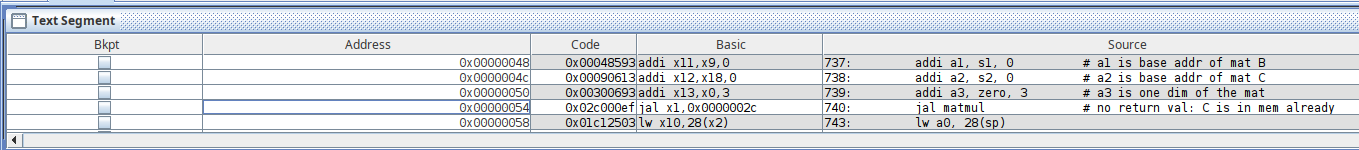
\includegraphics[width=0.8\textwidth]{./photos/rars_start.png}
				\caption{MatrixMult.asm Start Codes for PC}
				\label{fig:-photos-rars_start-png}
			\end{figure}

			\begin{figure}[H]
				\centering
				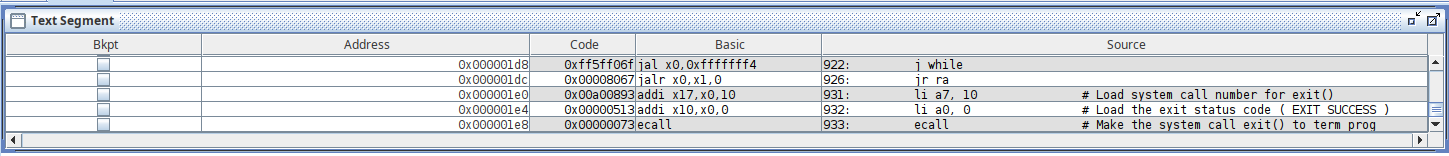
\includegraphics[width=0.8\textwidth]{./photos/rars_exit.png}
				\caption{MatrixMult.asm Exit Codes for PC}
				\label{fig:-photos-rars_exit-png}
			\end{figure}
			


			\subsubsection{TC 3x3}
				\begin{figure}[H]
					\centering
					
\includegraphics[width=0.8\textwidth]{./photos/m3/sim_before.png}
					\caption{Results Matrix "C" before instruction execution.}
					\label{fig:-photos-m3-}
				\end{figure}

				\begin{figure}[H]
					\centering
					
\includegraphics[width=0.8\textwidth]{./photos/m3/sim_timing.png}
					\caption{Waveform and Timing of TC 3x3 mat}
					\label{fig:-photos-m3-sim_timing-png}
				\end{figure}

				\begin{align*}
					 t_{execution} &= t_{end} - t_{start}\\
					 &= 107.730 \mu s - 2.290 \mu s \\
					 &= 105.44 \mu s \\
				 \end{align*}

				 \begin{align*}
					n_{CLK\_Cycles} &= \frac{t_{execution}}{T_{CLK}}\\
					&= \frac{105.44 \mu s}{10 ns} \\
					&= 10,544 \\
				 \end{align*}


				
			\subsubsection{TC 10x10}

				\begin{figure}[H]
					\centering
					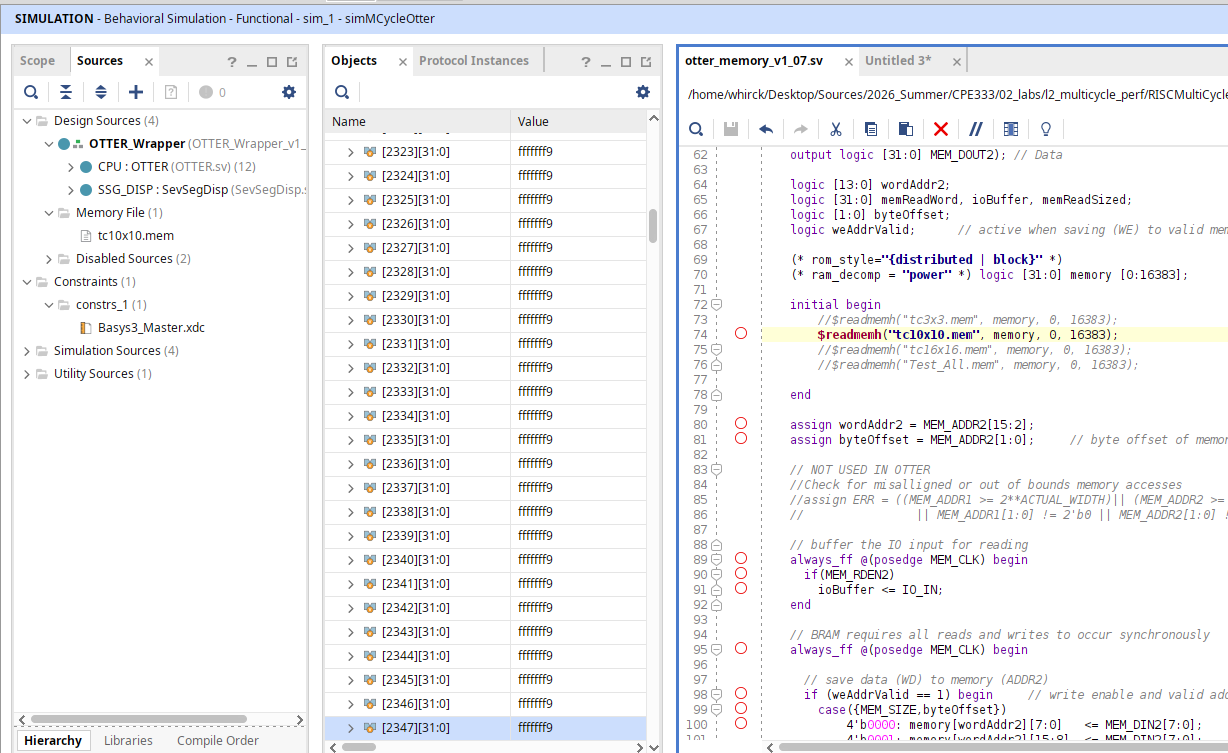
\includegraphics[width=0.8\textwidth]{./photos/m10/sim_before.png}
					\caption{Results Matrix "C" before instruction execution.}
					\label{fig:-photos-m3-}
				\end{figure}

				\begin{figure}[H]
					\centering
					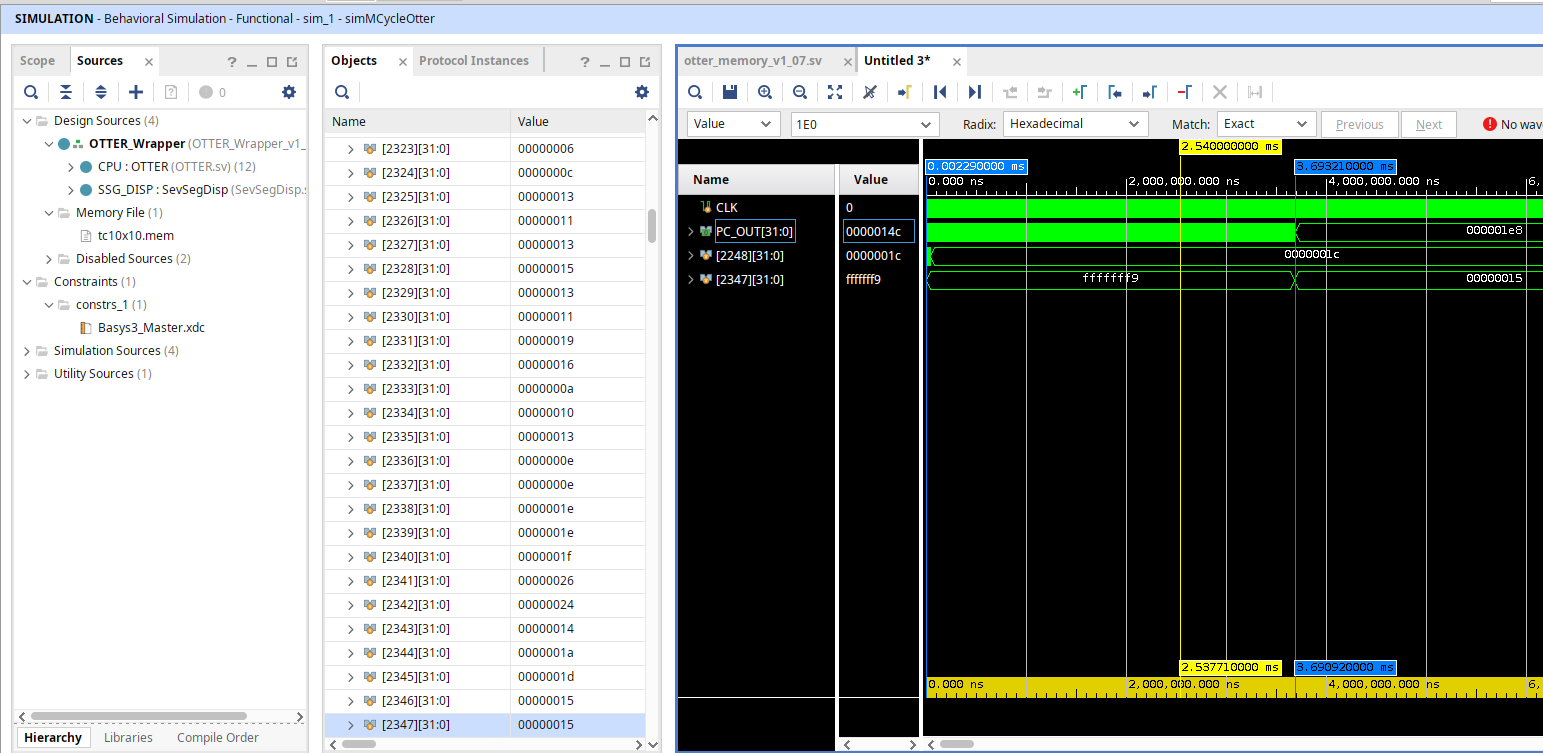
\includegraphics[width=0.8\textwidth]{./photos/m10/sim_timing.png}
					\caption{Waveform and Timing of TC 10x10 mat}
					\label{fig:-photos-m3-sim_timing-png}
				\end{figure}

				\begin{align*}
					 t_{execution} &= t_{end} - t_{start}\\
					 &= 3.69321 ms - 0.00229 ms \\
					 &= 3.69092 ms \\
				 \end{align*}

				 \begin{align*}
					n_{CLK\_Cycles} &= \frac{t_{execution}}{T_{CLK}}\\
					&= \frac{3.69092  ms}{10 ns} \\
					&= 369,092 \\
				 \end{align*}

			\subsubsection{TC 16x16}

				\begin{figure}[H]
					\centering
					
\includegraphics[width=0.8\textwidth]{./photos/m16/sim_before.png}
					\caption{Results Matrix "C" before instruction execution.}
					\label{fig:-photos-m3-}
				\end{figure}

				\begin{figure}[H]
					\centering
					
\includegraphics[width=0.8\textwidth]{./photos/m16/sim_timing.png}
					\caption{Waveform and Timing of TC 16x16 mat}
					\label{fig:-photos-m3-sim_timing-png}
				\end{figure}

				\begin{align*}
					 t_{execution} &= t_{end} - t_{start}\\
					 &= 14.82665 ms - 0.0022900 ms \\
					 &= 14.82436 ms \\
				 \end{align*}

				 \begin{align*}
					n_{CLK\_Cycles} &= \frac{t_{execution}}{T_{CLK}}\\
					&= \frac{14.82665  ms}{10 ns} \\
					&= 1,482,436 \\
				 \end{align*}

			\subsubsection{MatrixMult Summary}

				\begin{figure}[H]
					\centering
					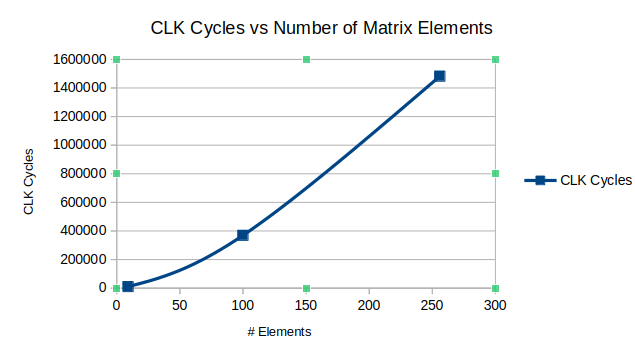
\includegraphics[width=0.8\textwidth]{./photos/rars_summary.png}
					\caption{CLK Cycles vs. Number of Elements in the Matrix}
					\label{fig:-photos-rars_summary-png}
				\end{figure}

				Power and utilization are the same for each matrix testcase.
				\begin{figure}[H]
					\centering
					
\includegraphics[width=0.6\textwidth]{./photos/m3/power.png}
					\caption{Power Summary}
					\label{fig:-photos-m3-power-png}
				\end{figure}

				\begin{figure}[H]
					\centering
					
\includegraphics[width=0.6\textwidth]{./photos/m3/util.png}
					\caption{Utilization Summary}
					\label{fig:-photos-m3-util-png}
				\end{figure}

				
	\newpage
	\section{Testall Performance}

		\subsection{Procedure}
			\begin{enumerate}
				\item Load the testall mem file onto the multicycle otter. 
						It should be noted that Diego's testall program 
						worked well such that the Basys3 board also gave LED 
						and sseg indicators that the system was working. 

				\item Capture the same waveforms, cpu execution time, power, 
						and area utilization. 
			\end{enumerate}

		\subsection{Results}

			\begin{figure}[H]
				\centering
				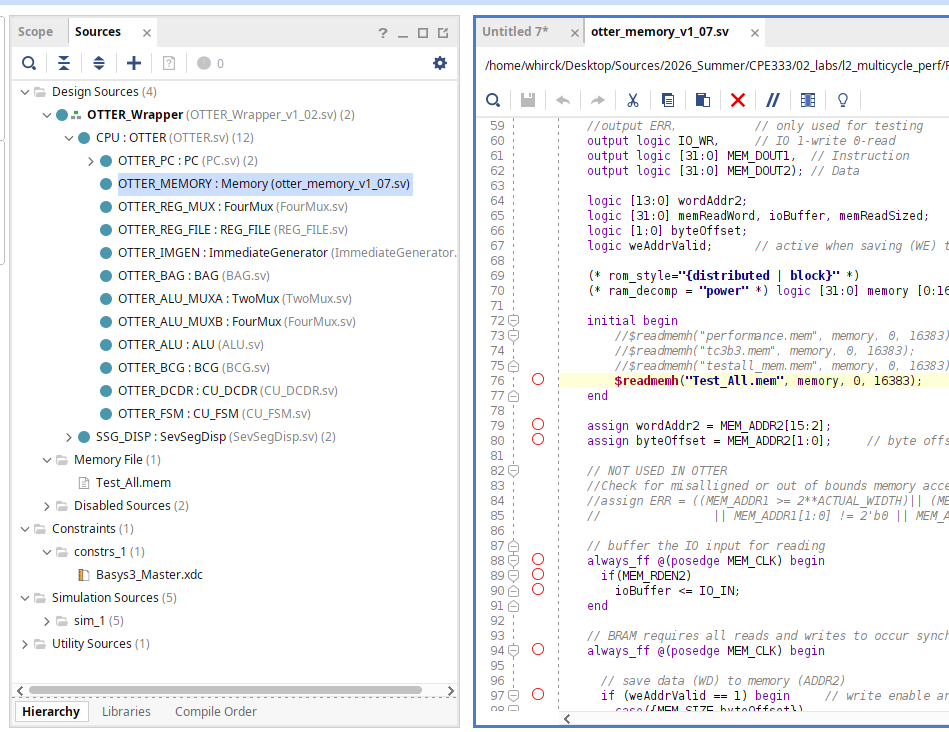
\includegraphics[width=0.8\textwidth]{./photos/testall_intro.png}
				\caption{Uploading the testall memory}
				\label{fig:-photos-testall_intro-png}
			\end{figure}

			\subsubsection{Timing}

				\begin{figure}[H]
					\centering
					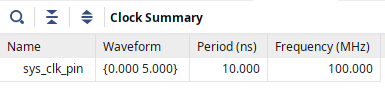
\includegraphics[width=0.6\textwidth]{./photos/testall_clk.png}
					\caption{Clock Speed}
					\label{fig:-photos-testall_clk-png}
				\end{figure}

				\begin{figure}[H]
					\centering
					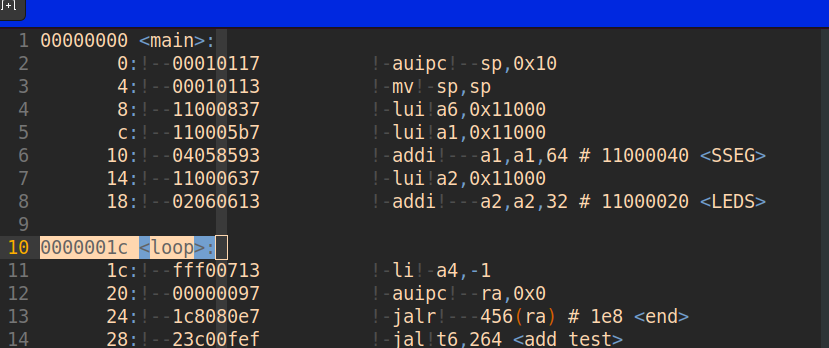
\includegraphics[width=0.8\textwidth]{./photos/testall_timing_target.png}
					\caption{Target Instruction Address for Timing Intervals in \textbf{Test\_All\_Debug.txt}}
					\label{fig:-photo-testall_timing}
				\end{figure}

				The \textit{loop} label was used for measurement because
				the testall program returns to this after running all tests.

				\begin{figure}[H]
					\centering
					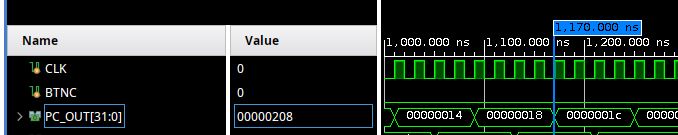
\includegraphics[width=0.8\textwidth]{./photos/testall_timing1.png}
					\caption{Measured Start Timestamp}
					\label{fig:-photos-testall_timing1}
				\end{figure}

				\begin{figure}[H]
					\centering
					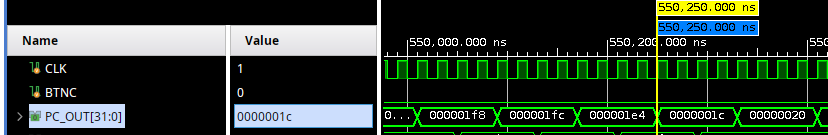
\includegraphics[width=0.8\textwidth]{./photos/testall_timing2.png}
					\caption{Measured End Timestamp}
					\label{fig:-photos-testall_timing2-png}
				\end{figure}

				 \begin{align*}
					 t_{execution} &= t_{end} - t_{start}\\
					 &= 550,250 ns - 1,170 ns \\
					 &= 549,080 ns \\
				 \end{align*}

				 \begin{align*}
					n_{CLK\_Cycles} &= \frac{t_{execution}}{T_{CLK}}\\
					&= \frac{549080 ns}{10 ns} \\
					&= 54,908 \\
				 \end{align*}

				 Note that the number above is not the number of instructions
				 executed. 

			\subsubsection{Other Metrics}
				\begin{figure}[H]
					\centering
					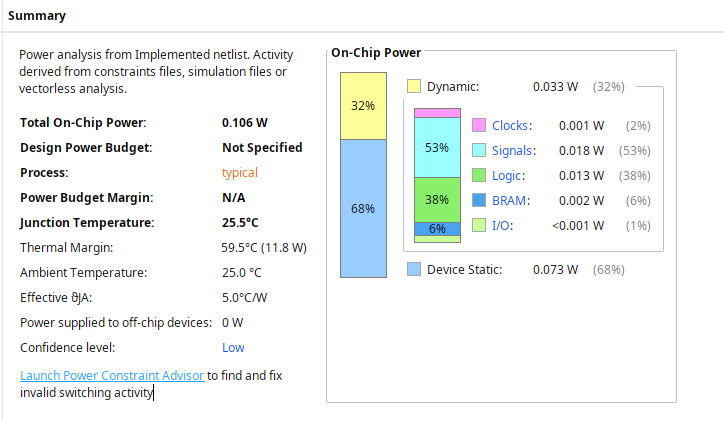
\includegraphics[width=0.8\textwidth]{./photos/testall_power.png}
					\caption{Power Summary of Testall on Basys3}
					\label{fig:-photos-testall_power}
				\end{figure}

				\begin{figure}[H]
					\centering
					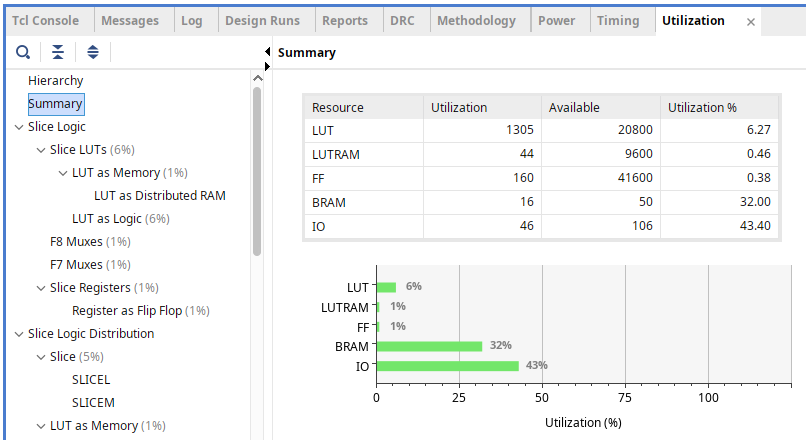
\includegraphics[width=0.8\textwidth]{./photos/testall_area2.png}
					\caption{Utilization Summary of Testall}
					\label{fig:-photos-testall_area2-png}
				\end{figure}
								
	\newpage
	\section{Notes}
		\subsection{RARS}
			\begin{figure}[H]
				\centering
				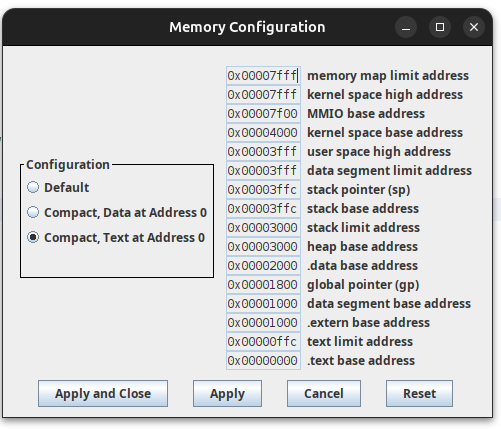
\includegraphics[width=0.6\textwidth]{./photos/rars_memconfig}
				\caption{RARS Memory Config Settings}
				\label{fig:-photos-rars_memconfig}
			\end{figure}

			\begin{figure}[H]
				\centering
				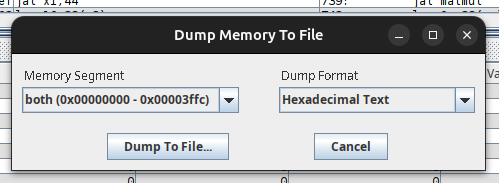
\includegraphics[width=0.6\textwidth]{./photos/rars_dumpconfig}
				\caption{RARS Memory Dump Config}
				\label{fig:-photos-rars_dumpconsig}
			\end{figure}

			\begin{figure}[H]
				\centering
				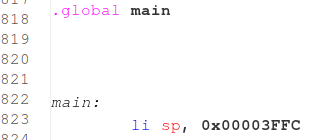
\includegraphics[width=0.6\textwidth]{./photos/rars_needed.png}
				\caption{Stack Pointer set after Data Segment}
				\label{fig:-photos-rars_needed-png}
			\end{figure}
			
\end{document}
